\documentclass[a4paper,10pt,twoside,openright]{book}
\usepackage[english]{babel}
\usepackage{graphicx}
\usepackage{subfigure}
\usepackage{subfloat}
%\usepackage{lineno}
\usepackage[usenames,dvipsnames,svgnames,table]{xcolor}
\definecolor{light-gray}{gray}{0.9}
\usepackage{afterpage}

\usepackage{dcolumn}
\newcolumntype{x}[1]{%
>{\centering\arraybackslash}m{#1}}%

\newcolumntype{L}[1]{>{\raggedright\arraybackslash}m{#1}}
\newcolumntype{R}[1]{>{\raggedleft\arraybackslash}m{#1}}
%\newcolumntype{L}[1]{>{\raggedright\let\newline\\\arraybackslash\hspace{0pt}}m{#1}}
%\newcolumntype{C}[1]{>{\centering\let\newline\\\arraybackslash\hspace{0pt}}m{#1}}
%\newcolumntype{R}[1]{>{\raggedleft\let\newline\\\arraybackslash\hspace{0pt}}m{#1}

\usepackage[percent]{overpic}

\newcommand{\nocontentsline}[3]{}
\newcommand{\tocless}[2]{\bgroup\let\addcontentsline=\nocontentsline#1{#2}\egroup}

\usepackage{multirow,bigdelim}
\usepackage{enumerate}

\usepackage[margin=7pt,font=small,labelfont=bf]{caption}
\usepackage{booktabs}
\usepackage{longtable}
\usepackage{lscape}

%SOME SYMBOLS
\usepackage{pifont}
\newcommand{\cmark}{\ding{51}}%
\newcommand{\xmark}{\ding{55}}%
%MATHS
\usepackage{amssymb}
\usepackage{amsmath}
\usepackage{latexsym}
\usepackage{amsthm}
 \newcommand{\sgn}{\mathop{\mathrm{sgn}}}
\usepackage{slashed}

\usepackage{listings}
\lstset{language=C}

\hyphenation{ca-lo-ri-me-ter ca-lo-ri-me-ters}%serve per la sillabazione: tra parentesi 

\setlength{\headheight}{15pt}
\usepackage{pict2e}

\usepackage{eso-pic}

\usepackage{url}
%%%%bookmarksnumbered=false,% true means bookmarks in left window are numbered
%%%%dvips,%ps2pdf,
%%%%bookmarksopen=false, % true means only level 1 are displayed.
%%%%breaklinks=true,linktocpage
\usepackage[breaklinks=true,linktocpage,ocgcolorlinks,bookmarks=true,bookmarksnumbered=false,bookmarksopen=false,colorlinks=true,linkcolor=webred]{hyperref}
%\usepackage[bookmarks=true,bookmarksnumbered=false,bookmarksopen=false]{hyperref}
%\usepackage[pdfborder={0 0 0 0}]{hyperref}
\definecolor{webgreen}{rgb}{0, 0.5, 0} % less intense green
\definecolor{webblue}{rgb}{0, 0, 0.5} % less intense blue
\definecolor{webred}{rgb}{0.5, 0, 0} % less intense red

\usepackage[hdivide={2cm, *, 2cm}, vscale=0.85]{geometry}
\usepackage{chngpage}
\usepackage{setspace}


\usepackage{fancyhdr}
\pagestyle{fancy}



%per avere l'indice senza numeri di pagina
\makeatletter 
 \newcommand{\cleantableofcontents}{% 
   \clearpage\begingroup 
   \let\ps@plain\ps@empty\pagestyle{empty}% 
   \tableofcontents\clearpage\endgroup} 
 \makeatother

%per lo stile dei capitoli
\makeatletter
\def\thickhrulefill{\leavevmode \leaders \hrule height 1ex \hfill \kern \z@}
%chstyle
\def\@makechapterhead#1{%
  \vspace*{10\p@}%
  {\parindent \z@ 
    {\raggedleft \reset@font
      \scshape \@chapapp{} \thechapter\par\nobreak}%
    \par\nobreak
    \vspace*{30\p@}
    \interlinepenalty\@M
    {\begin{spacing}{1.1} \raggedright \huge \bfseries #1\end{spacing}}%
    %{\doublespacing \raggedright \huge \bfseries #1}%
    \par\nobreak
    \hrulefill
    \par\nobreak
    \vskip 90\p@
  }}
\def\@makeschapterhead#1{%
  \vspace*{10\p@}%
  {\parindent \z@ 
    {\raggedleft \reset@font
      \scshape \vphantom{\@chapapp{} \thechapter}\par\nobreak}%
    \par\nobreak
    \vspace*{30\p@}
    \interlinepenalty\@M
    {\begin{spacing}{1.1} \raggedright \huge \bfseries #1\end{spacing}}%
    \par\nobreak
    \hrulefill
    \par\nobreak
    \vskip 90\p@
  }}


\renewcommand{\chaptermark}[1]{\markboth{\thechapter. \ #1}{}}
\renewcommand{\sectionmark}[1]{\markright{\thesection.\ #1}}
\fancyhf{}
\fancyhead[LO]{\small \nouppercase{\rightmark}}
\fancyhead[RE]{\small \nouppercase{\leftmark}}
\fancyhead[RO , LE]{ \thepage}



%%%%%%%%%%%%%%%%%%
%%% LAAAAAZYYYYY
%%%%%%%%%%%%%%%%%%
\def\bxii{B\ensuremath{_{12}}}



\begin{document}


\frontmatter


\pdfbookmark[1]{Index}{Index}
\cleantableofcontents

\clearpage{\pagestyle{empty}\cleardoublepage}
\mainmatter

\chapter{Data Science Toolbox}

\href{https://www.coursera.org/course/datascitoolbox}{Coursera} classes, Feb 3rd - Mar 8th 2015. 
Examples of Data Science (DS) problems are:
\begin{itemize}
\item descriptive: simply describe data, like population census, no generalization is possible;
\item exploratory: look for connections and correlations in data, but {\it correlation does not imply causation}!;
\item inferential: extrapolate information from small sample to large population;
\item predictive: use data on one object to predict effect on another object ({\it prediction is very hard especially about the future!});
\item causal: identify causal relationships between variables (changes on one variable caused by changes on another variable);
\item mechanistic: find exact changes in variables leading to changes in another variable.
\end{itemize}

Confounding variable:

%\section{Statistical data science}



\section{R}

To start:
\begin{itemize}
\item \url{http://www.r-project.org/}: official page for \texttt{R}
\item \url{http://www.rstudio.com/}: according to many one of the best IDE\dots will see!
\item \href{http://cran.r-project.org/}{CRAN}: the Comprehensive R Archive Network, to look for packages
\item \href{http://www.bioconductor.org/}{Bioconductor Project}: packages for biological applications, wohoo!
\end{itemize}
Under CRAN Task Views packages related to various topics are grouped.
To install, load and see which functions are available in a package do:
\begin{lstlisting}[language=R]
install.packages(``pckgname'')
library(pckgname)
search()
\end{lstlisting}
To install packages from Bioconductor do:
\begin{lstlisting}[language=R]
source(``http://www.bioconductor.org/biocLite.R'')
biocLite()
biocLite(c(``pckg1'', ``pckg2'', ``pckg3''))
\end{lstlisting}

RmySQL

Building data products: R packages; rCharts; Shiny


\section{Git and GitHub}

To configure git with the github username and email:
\begin{lstlisting}[language=bash]
git config --global user.name asuccurro
git config --global user.email a.succurro@gmail.com
\end{lstlisting}
To avoid re-entering always user name and password in short time set a higher cache time:
\begin{lstlisting}[language=bash]
git config --global credential.helper 'cache --timeout=3600'
\end{lstlisting}
Whenever a ``new-repo'' is created, go to the chosen local \texttt{new-repo} and do:
\begin{lstlisting}[language=bash]
git init
git remote add origin https://github.com/asuccurro/new-repo.git
\end{lstlisting}
To add new files and commit and push to the remote github:
\begin{lstlisting}[language=bash]
git add stuff stuff morestuff
git commit -m 'message'
git push origin master
\end{lstlisting}
To commit all the modified files:
\begin{lstlisting}[language=bash]
git commit -am 'message'
\end{lstlisting}
Branching is used to modify a parallel version of the project. To switch to the branch called ``branchname'':
\begin{lstlisting}[language=bash]
git checkout -b branchname
\end{lstlisting}
To switch back to the master:
\begin{lstlisting}[language=bash]
git checkout master
\end{lstlisting}
To check where you are:
\begin{lstlisting}[language=bash]
git branch
\end{lstlisting}

\begin{lstlisting}[language=bash]
\end{lstlisting}

\begin{lstlisting}[language=bash]
\end{lstlisting}

\begin{lstlisting}[language=bash]
\end{lstlisting}

\begin{lstlisting}[language=bash]
\end{lstlisting}


To ``fork'' a project, go to the project github and click on the fork: this will simply copy the current version of the project
into the personal github. Then the copied project can be pulled:
\begin{lstlisting}[language=bash]
\end{lstlisting}



\begin{figure}[htb]\begin{center}
\subfigure[]{\label{fig:gitflow}
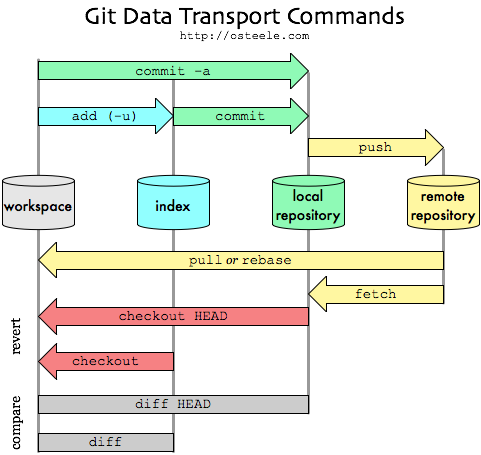
\includegraphics[width=0.5\textwidth]{00_datascientisttoolbox/pics/git-transport}}
\caption{From \href{http://gitready.com/beginner/2009/01/21/pushing-and-pulling.html}{gitready}.}
\end{center}\end{figure}




\chapter{R programming}

\href{https://class.coursera.org/rprog-016/}{Coursera} classes

{\it Programming with Data} by John Chambers - originally was the \texttt{S} language: \texttt{R} is a ``dialect'' of \texttt{S}. 
{\it Software for Data Analysis} by John Chambers (Springer, 2008)

Assignement operator: \href{http://stackoverflow.com/questions/1741820/assignment-operators-in-r-and}{stackoverflow}


\begin{lstlisting}
> x <- c(3, 5, 1, 10, 12, 6)
> x[x %in% 1:5] <- 0
\end{lstlisting}


\begin{figure}[htb]\begin{center}
\subfigure[]{\label{fig:types}
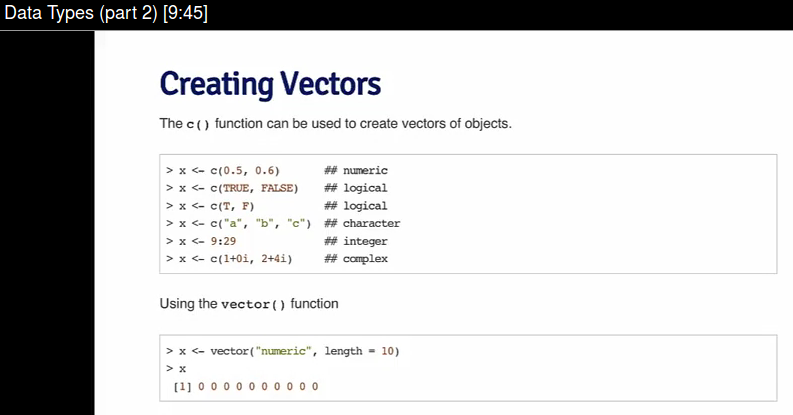
\includegraphics[width=0.45\textwidth]{01_rprogramming/pics/data_types.png}}
\subfigure[]{\label{fig:matrix}
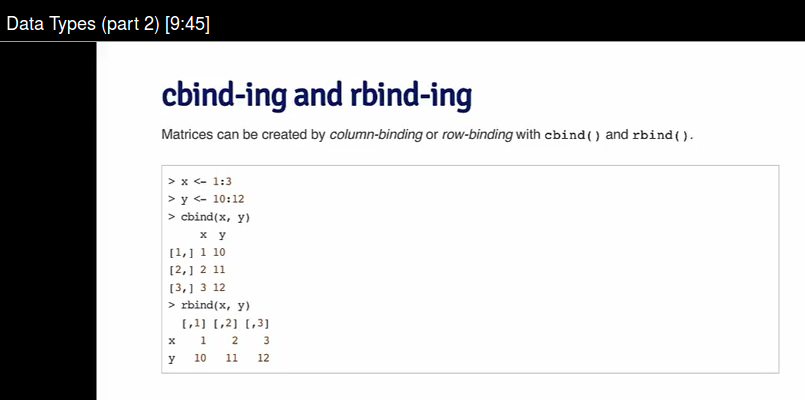
\includegraphics[width=0.45\textwidth]{01_rprogramming/pics/matrixbind.png}}
\caption{(a) Available data types: numerical, integer (1 = numerical, 1L = integer), complex, logical, character. Single elements are vector! (b) Build matrices binding
vectors as rows or columns.}
\end{center}\end{figure}



\begin{figure}[htb]\begin{center}
\subfigure[]{\label{fig:lists}
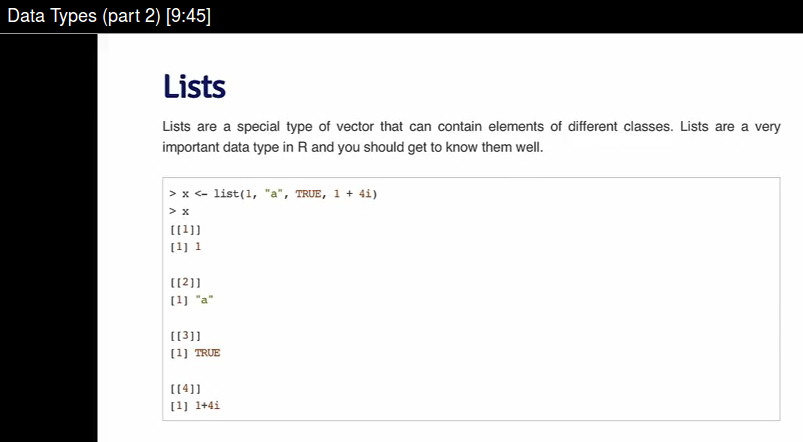
\includegraphics[width=0.45\textwidth]{01_rprogramming/pics/lists.png}}
\subfigure[]{\label{fig:factors}
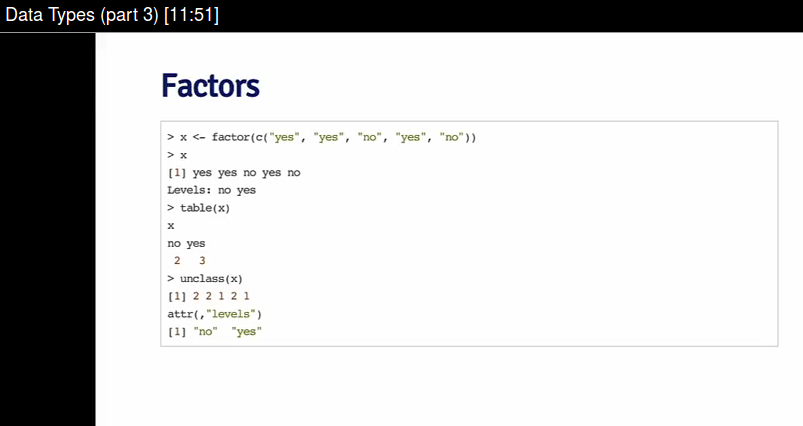
\includegraphics[width=0.45\textwidth]{01_rprogramming/pics/factors.png}}
\caption{(a) Vectors element are always of the same type, eventually the type is re-assigned. Lists can contain different types, are accessed with $[[]]$. 
(b) Factors represent {\bf categorical data} and basically label integer flags. Levels (= list of flags) are authomatically ordered alphabetically! 
To avoid this and have the base level desired add \texttt{, levels = c(``yes'', ``no'')}}
\end{center}\end{figure}



\begin{figure}[htb]\begin{center}
\subfigure[]{\label{fig:frames}
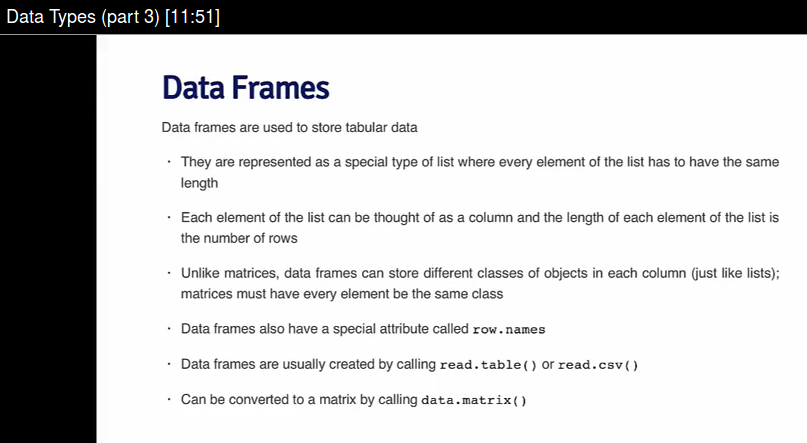
\includegraphics[width=0.45\textwidth]{01_rprogramming/pics/dataframes.png}}
\subfigure[]{\label{fig:names}
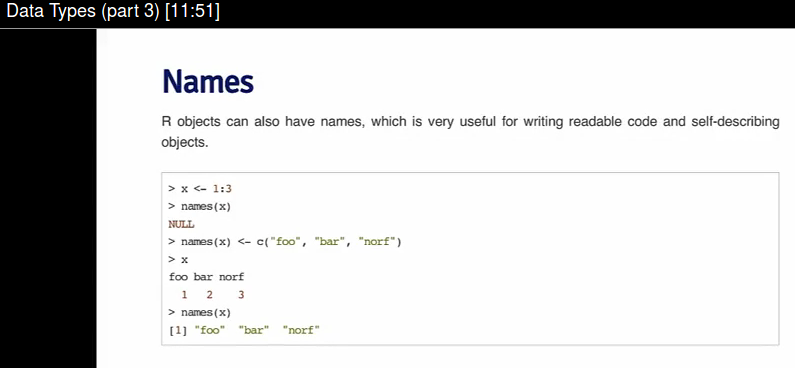
\includegraphics[width=0.45\textwidth]{01_rprogramming/pics/names}}
\caption{}
\end{center}\end{figure}


\begin{figure}[htb]\begin{center}
\subfigure[]{\label{fig:}
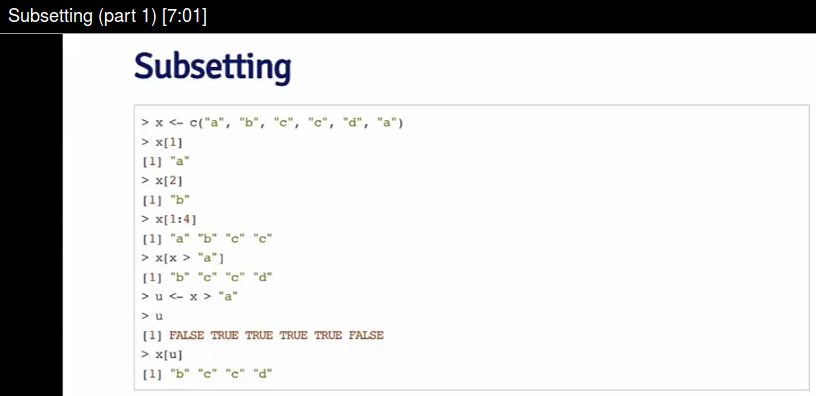
\includegraphics[width=0.45\textwidth]{01_rprogramming/pics/subset1}}
\subfigure[]{\label{fig:}
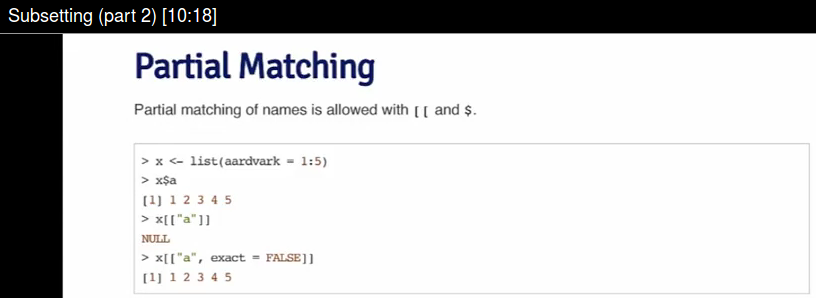
\includegraphics[width=0.45\textwidth]{01_rprogramming/pics/subset2}}
\caption{}
\end{center}\end{figure}

\begin{figure}[htb]\begin{center}
\subfigure[]{\label{fig:}
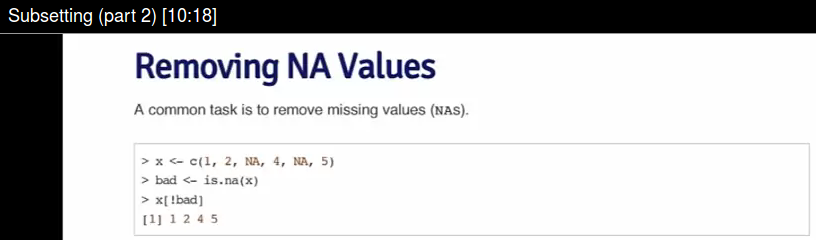
\includegraphics[width=0.45\textwidth]{01_rprogramming/pics/subset3}}
\subfigure[]{\label{fig:}
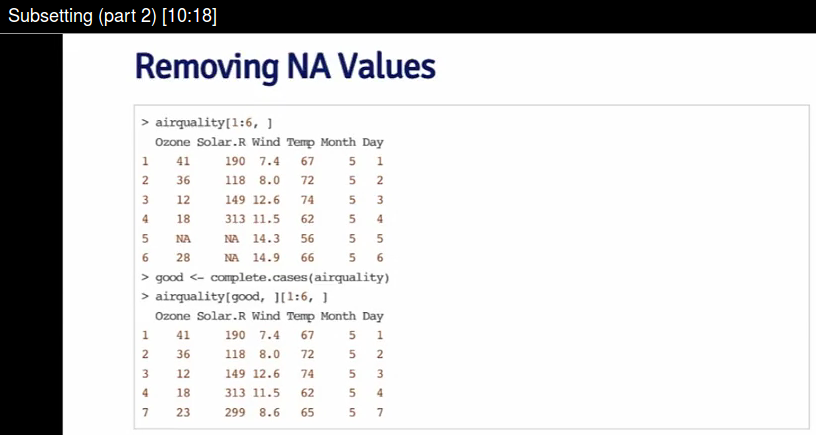
\includegraphics[width=0.45\textwidth]{01_rprogramming/pics/subset4}}
\caption{}
\end{center}\end{figure}

\begin{figure}[htb]\begin{center}
\subfigure[]{\label{fig:}
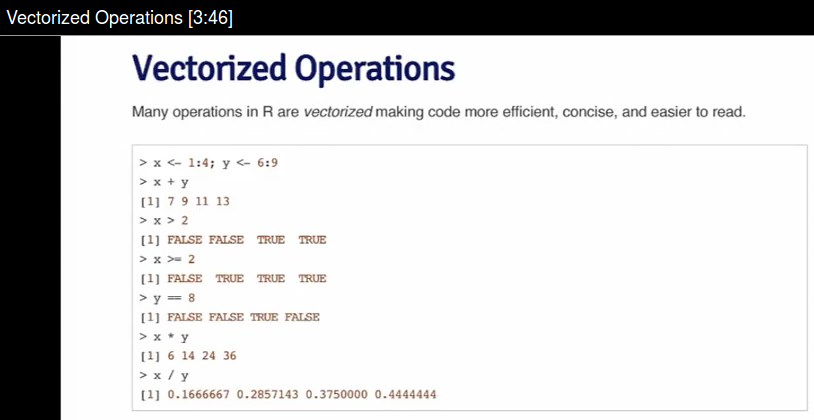
\includegraphics[width=0.45\textwidth]{01_rprogramming/pics/subset5}}
\subfigure[]{\label{fig:}
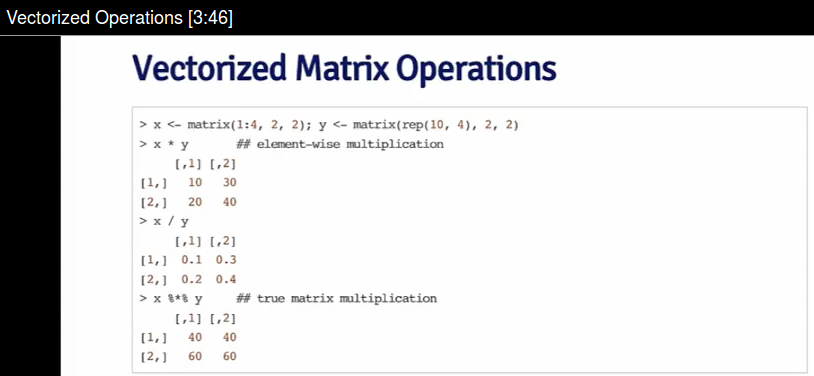
\includegraphics[width=0.45\textwidth]{01_rprogramming/pics/subset6}}
\caption{}
\end{center}\end{figure}

\begin{figure}[htb]\begin{center}
\subfigure[]{\label{fig:}
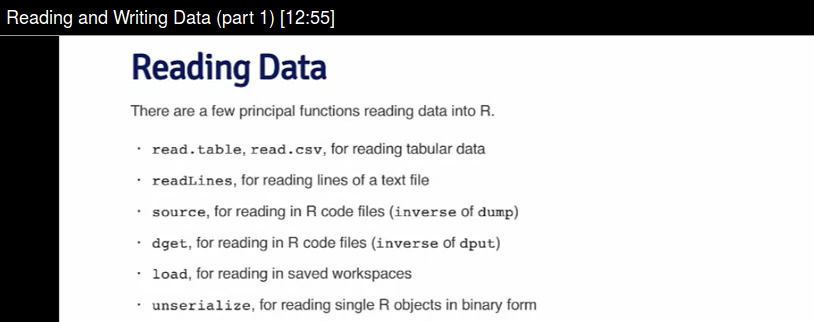
\includegraphics[width=0.45\textwidth]{01_rprogramming/pics/readingdata1}}
\subfigure[]{\label{fig:}
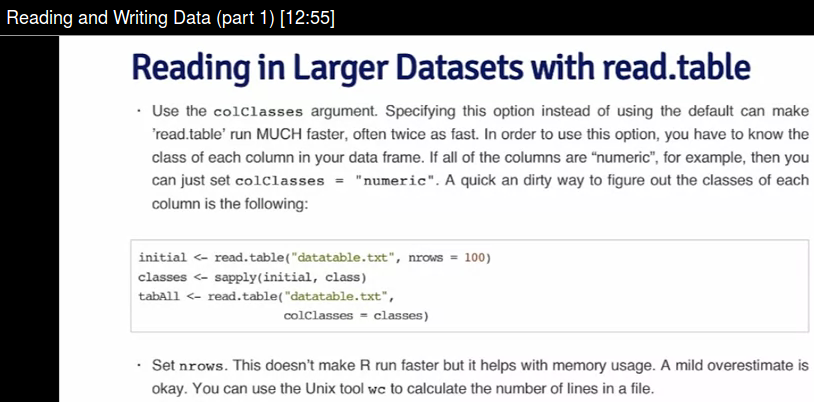
\includegraphics[width=0.45\textwidth]{01_rprogramming/pics/readingdata2}}
\caption{}
\end{center}\end{figure}

\begin{figure}[htb]\begin{center}
\subfigure[]{\label{fig:}
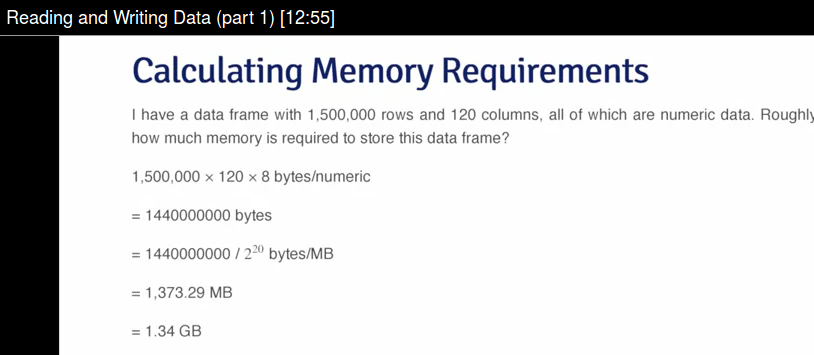
\includegraphics[width=0.45\textwidth]{01_rprogramming/pics/readingdata3}}
\subfigure[]{\label{fig:}
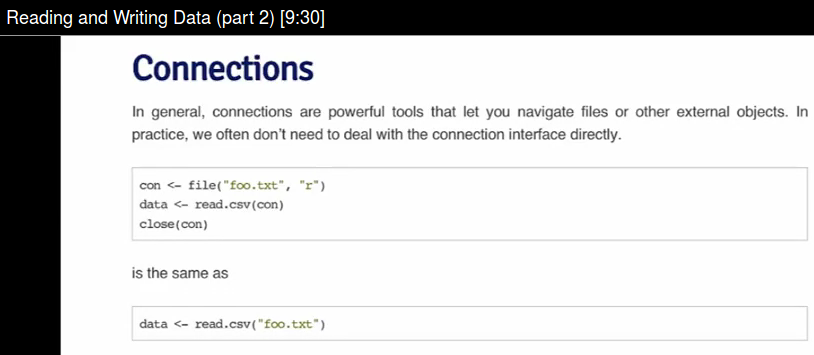
\includegraphics[width=0.45\textwidth]{01_rprogramming/pics/readingdata4}}
\caption{}
\end{center}\end{figure}

\begin{figure}[htb]\begin{center}
\subfigure[]{\label{fig:}
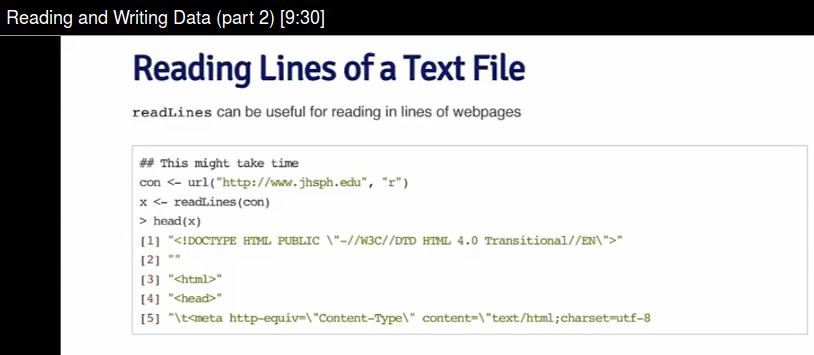
\includegraphics[width=0.45\textwidth]{01_rprogramming/pics/readingdata5}}
\subfigure[]{\label{fig:}
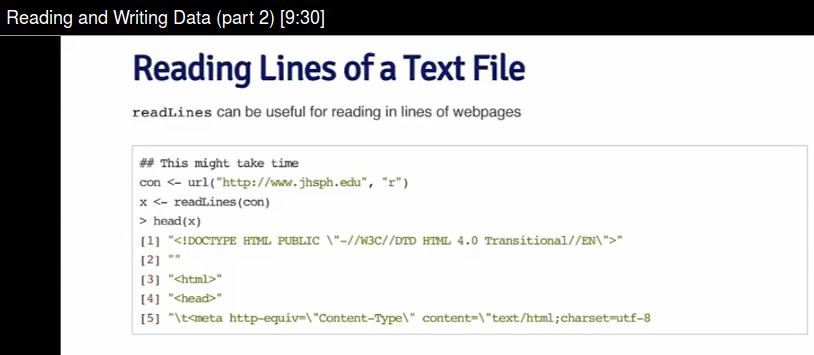
\includegraphics[width=0.45\textwidth]{01_rprogramming/pics/readingdata5}}
\caption{}
\end{center}\end{figure}


%\chapter{R programming}

\href{https://class.coursera.org/rprog-016/}{Coursera} classes

{\it Programming with Data} by John Chambers - originally was the \texttt{S} language: \texttt{R} is a ``dialect'' of \texttt{S}. 
{\it Software for Data Analysis} by John Chambers (Springer, 2008)

Assignement operator: \href{http://stackoverflow.com/questions/1741820/assignment-operators-in-r-and}{stackoverflow}


\begin{lstlisting}
> x <- c(3, 5, 1, 10, 12, 6)
> x[x %in% 1:5] <- 0
\end{lstlisting}


\begin{figure}[htb]\begin{center}
\subfigure[]{\label{fig:types}
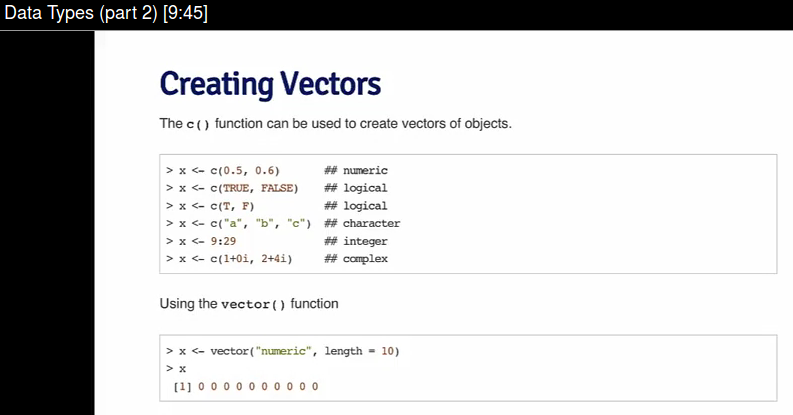
\includegraphics[width=0.45\textwidth]{01_rprogramming/pics/data_types.png}}
\subfigure[]{\label{fig:matrix}
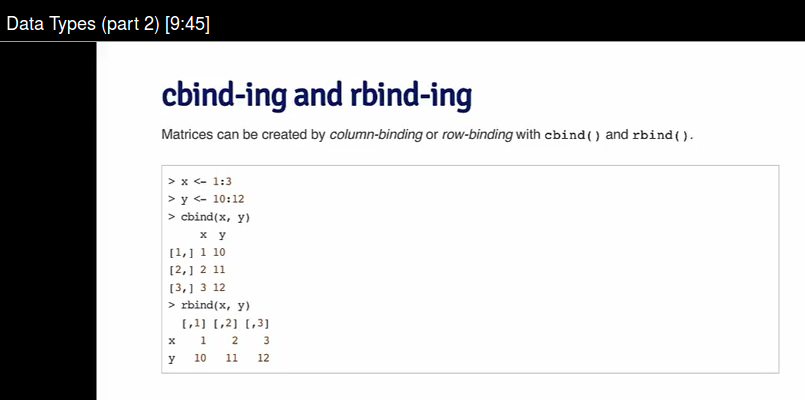
\includegraphics[width=0.45\textwidth]{01_rprogramming/pics/matrixbind.png}}
\caption{(a) Available data types: numerical, integer (1 = numerical, 1L = integer), complex, logical, character. Single elements are vector! (b) Build matrices binding
vectors as rows or columns.}
\end{center}\end{figure}



\begin{figure}[htb]\begin{center}
\subfigure[]{\label{fig:lists}
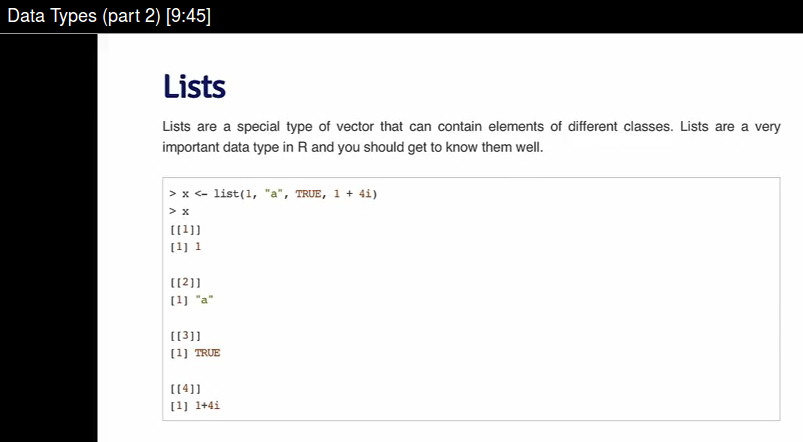
\includegraphics[width=0.45\textwidth]{01_rprogramming/pics/lists.png}}
\subfigure[]{\label{fig:factors}
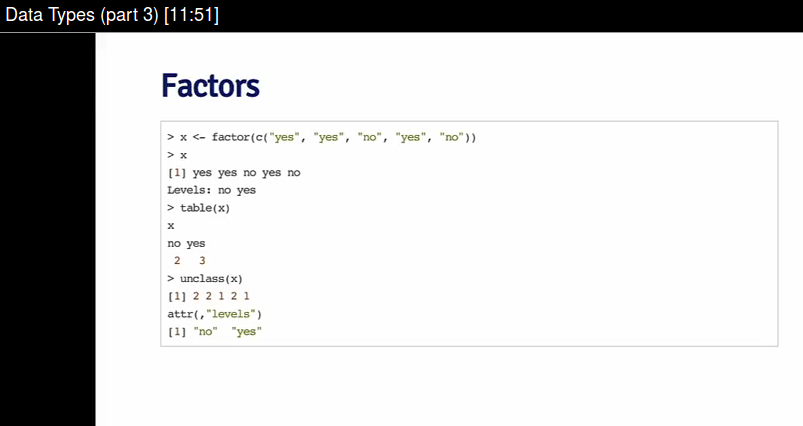
\includegraphics[width=0.45\textwidth]{01_rprogramming/pics/factors.png}}
\caption{(a) Vectors element are always of the same type, eventually the type is re-assigned. Lists can contain different types, are accessed with $[[]]$. 
(b) Factors represent {\bf categorical data} and basically label integer flags. Levels (= list of flags) are authomatically ordered alphabetically! 
To avoid this and have the base level desired add \texttt{, levels = c(``yes'', ``no'')}}
\end{center}\end{figure}



\begin{figure}[htb]\begin{center}
\subfigure[]{\label{fig:frames}
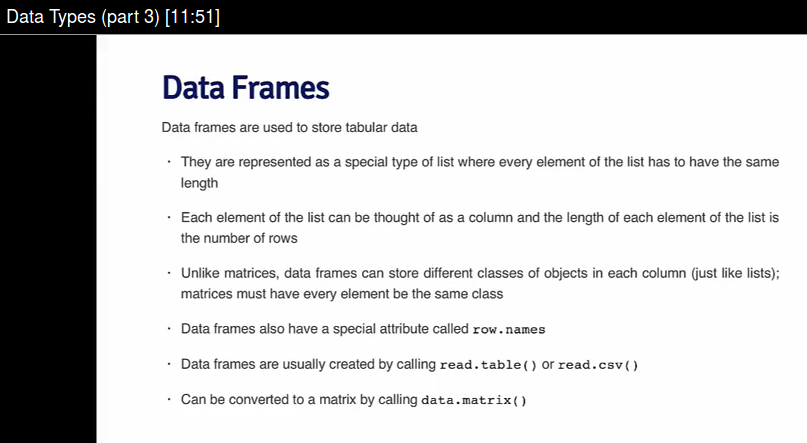
\includegraphics[width=0.45\textwidth]{01_rprogramming/pics/dataframes.png}}
\subfigure[]{\label{fig:names}
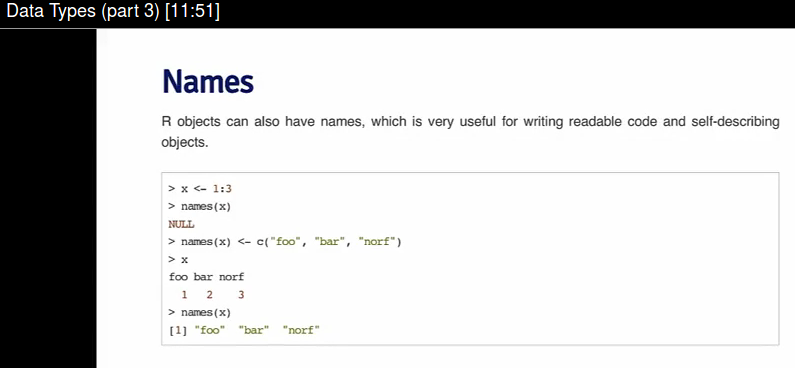
\includegraphics[width=0.45\textwidth]{01_rprogramming/pics/names}}
\caption{}
\end{center}\end{figure}


\begin{figure}[htb]\begin{center}
\subfigure[]{\label{fig:}
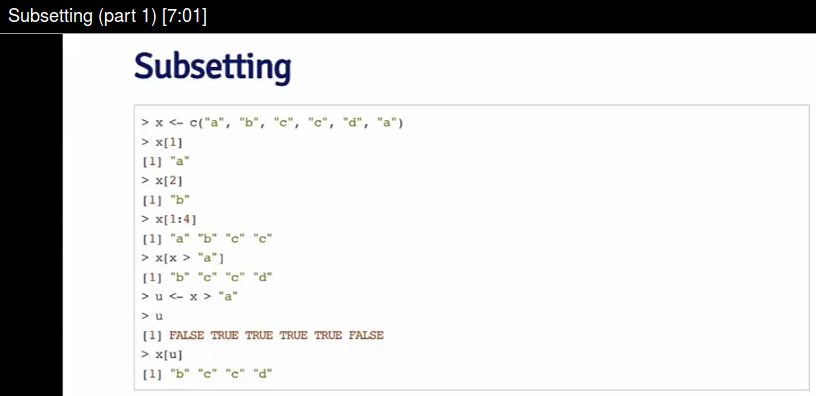
\includegraphics[width=0.45\textwidth]{01_rprogramming/pics/subset1}}
\subfigure[]{\label{fig:}
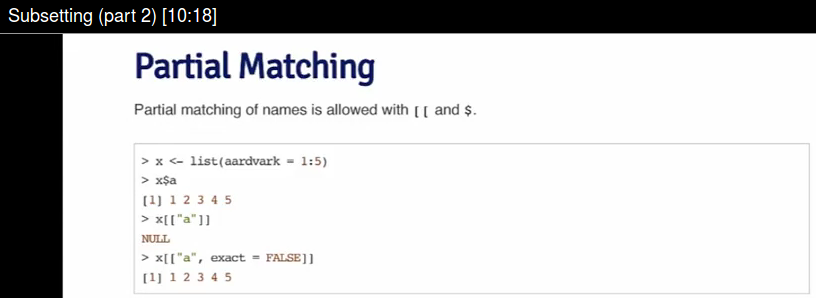
\includegraphics[width=0.45\textwidth]{01_rprogramming/pics/subset2}}
\caption{}
\end{center}\end{figure}

\begin{figure}[htb]\begin{center}
\subfigure[]{\label{fig:}
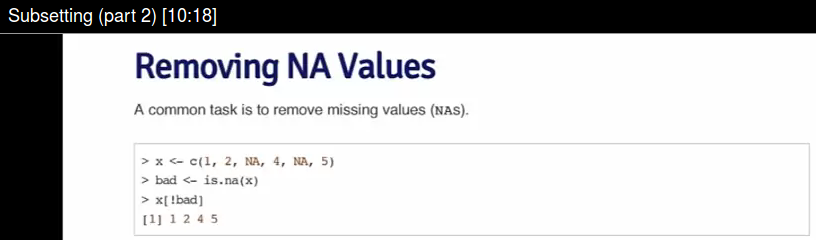
\includegraphics[width=0.45\textwidth]{01_rprogramming/pics/subset3}}
\subfigure[]{\label{fig:}
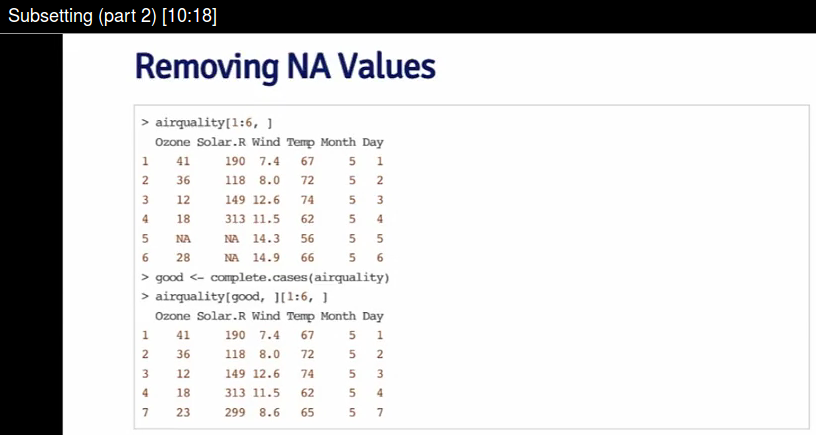
\includegraphics[width=0.45\textwidth]{01_rprogramming/pics/subset4}}
\caption{}
\end{center}\end{figure}

\begin{figure}[htb]\begin{center}
\subfigure[]{\label{fig:}
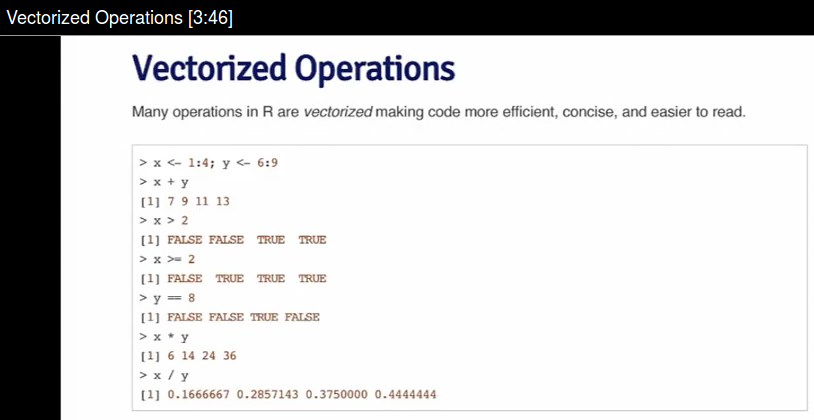
\includegraphics[width=0.45\textwidth]{01_rprogramming/pics/subset5}}
\subfigure[]{\label{fig:}
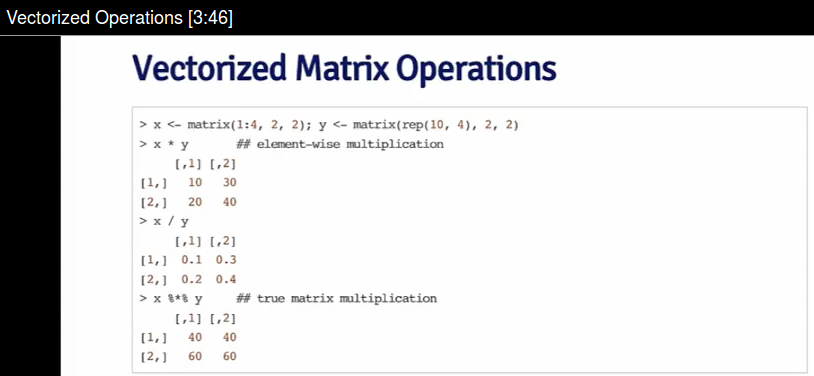
\includegraphics[width=0.45\textwidth]{01_rprogramming/pics/subset6}}
\caption{}
\end{center}\end{figure}

\begin{figure}[htb]\begin{center}
\subfigure[]{\label{fig:}
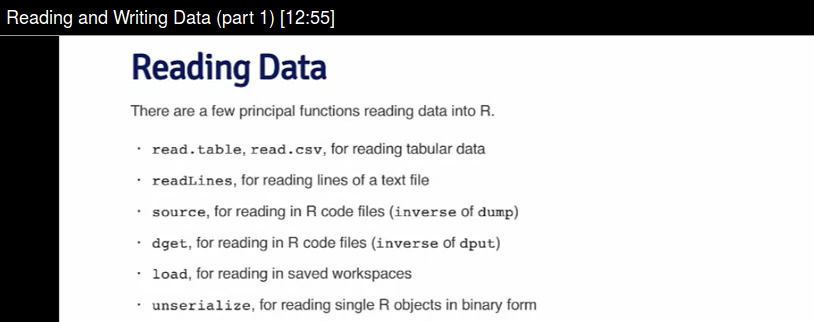
\includegraphics[width=0.45\textwidth]{01_rprogramming/pics/readingdata1}}
\subfigure[]{\label{fig:}
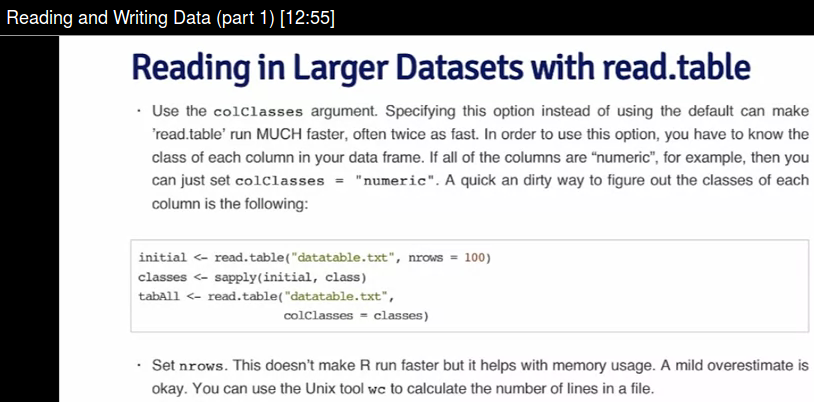
\includegraphics[width=0.45\textwidth]{01_rprogramming/pics/readingdata2}}
\caption{}
\end{center}\end{figure}

\begin{figure}[htb]\begin{center}
\subfigure[]{\label{fig:}
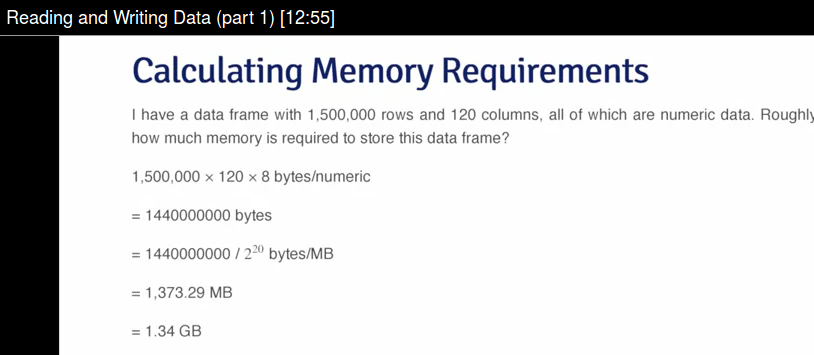
\includegraphics[width=0.45\textwidth]{01_rprogramming/pics/readingdata3}}
\subfigure[]{\label{fig:}
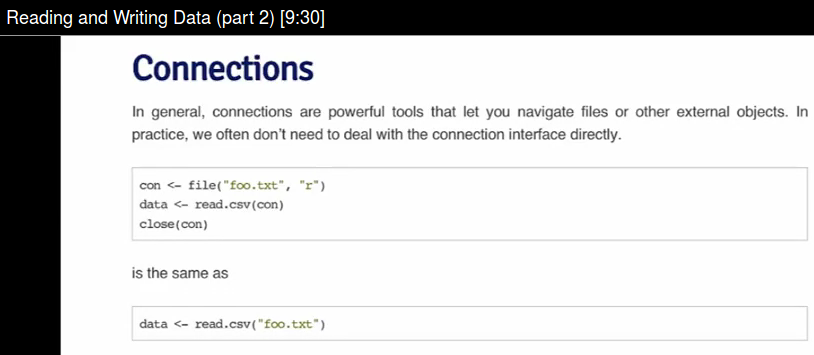
\includegraphics[width=0.45\textwidth]{01_rprogramming/pics/readingdata4}}
\caption{}
\end{center}\end{figure}

\begin{figure}[htb]\begin{center}
\subfigure[]{\label{fig:}
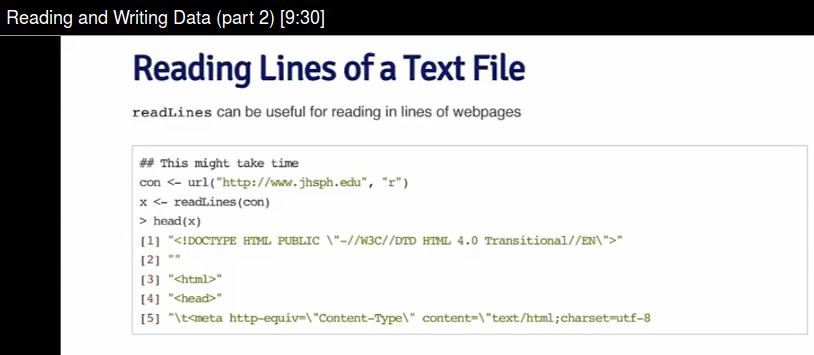
\includegraphics[width=0.45\textwidth]{01_rprogramming/pics/readingdata5}}
\subfigure[]{\label{fig:}
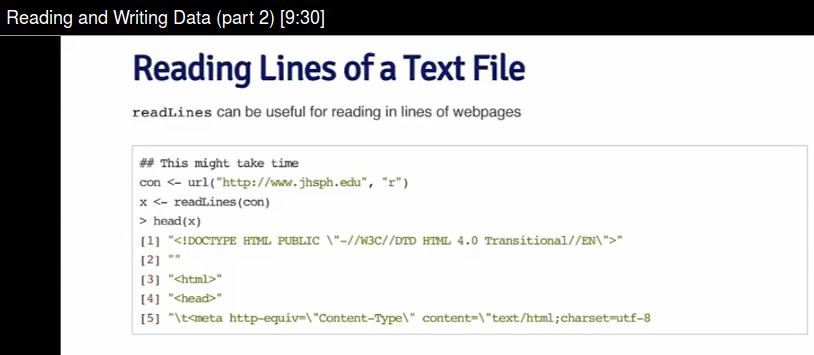
\includegraphics[width=0.45\textwidth]{01_rprogramming/pics/readingdata5}}
\caption{}
\end{center}\end{figure}


\appendix

%\input{}

\backmatter
%\nocite{}
%\phantomsection
%\addcontentsline{toc}{chapter}{Bibliography}
%\bibliographystyle{unsrt}
%\bibliographystyle{apalike}
%\bibliography{biblioB12}
%\clearpage{\pagestyle{empty}\cleardoublepage}

\end{document}
